\documentclass[xcolor=svgnames,14pt]{beamer}
\usepackage[utf8]{inputenc}
\usepackage[czech]{babel}
\usepackage{color}
\usepackage{graphicx,verbatim}

\usetheme{Parasim}

\title[Parasim]{Parasim: Nástroj pro paralelní simulaci a verifikaci}
\author{Jan Papoušek, Tomáš Vejpustek}
\institute{}
\date{23.\,Května 2013}

\begin{document}

\frame[plain]{\titlepage}

\begin{frame}{Úvod}
	\begin{itemize}
		\item Laboratoř systémové biologie (Sybila)
		\item analýza biologických modelů (zadané v~ODE)
		\item průzkum, jak je chování ovlivněno změnami modelu
	\end{itemize}
\end{frame}

\begin{frame}{Parametry}
	$$\frac{dX}{dt}=\nu X-\alpha XY	\qquad	\frac{dY}{dt}=\alpha XY-\mu Y$$
	\begin{description}
		\item[proměnné] ($X$, $Y$) -- počáteční hodnoty
		\item[koeficienty] ($\mu$, $\nu$, $\alpha$)
	\end{description}
	\begin{itemize}
		\item jak jejich změna ovlivní chování modelu?
		\item splňuje chování danou vlastnost?\\
			(temporální logiky)
	\end{itemize}
\end{frame}

\begin{frame}{Cíl analýzy}
	\begin{center}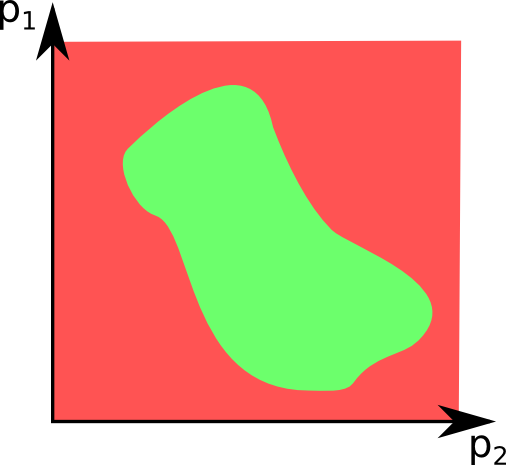
\includegraphics[height=0.7\textheight]{paramspace.png}\end{center}
\end{frame}

\begin{frame}{Spojitá doména}
	\begin{itemize}
		\item problém spojité domény\\$\implies$ aproximace -- samplování
		\item jak hustě samplovat? kde samplovat?
		\item heuristika řešení samplování
	\end{itemize}
\end{frame}

\begin{frame}{Výsledek analýzy}
	\centering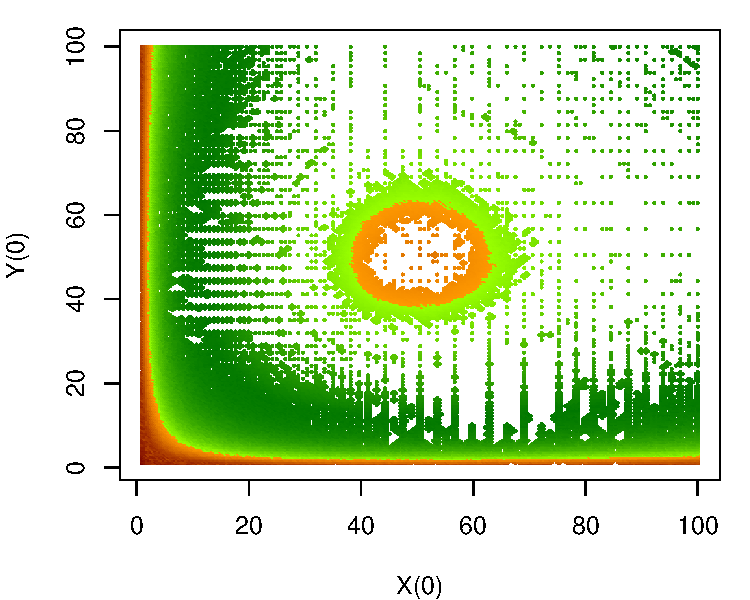
\includegraphics[width=0.9\textwidth]{lotkav-analysis.pdf}
\end{frame}

\begin{frame}{Parasim}
	\begin{itemize}
		\item modulární architektura -- snadné nahrazení novou implementací (vstup třetí strany)
		\item paralelizace
		\item GUI pro správu experimentů a vizualizaci výsledků (více dimenzí)
		\item založený na volně dostupných technologiích
	\end{itemize}
\end{frame}

\begin{frame}{Screenshot}
	\centering
\includegraphics[width=\textwidth]{../screenshots/parasim.png}
\end{frame}

\begin{frame}{Škálovatelnost (multicore)}
	\begin{center}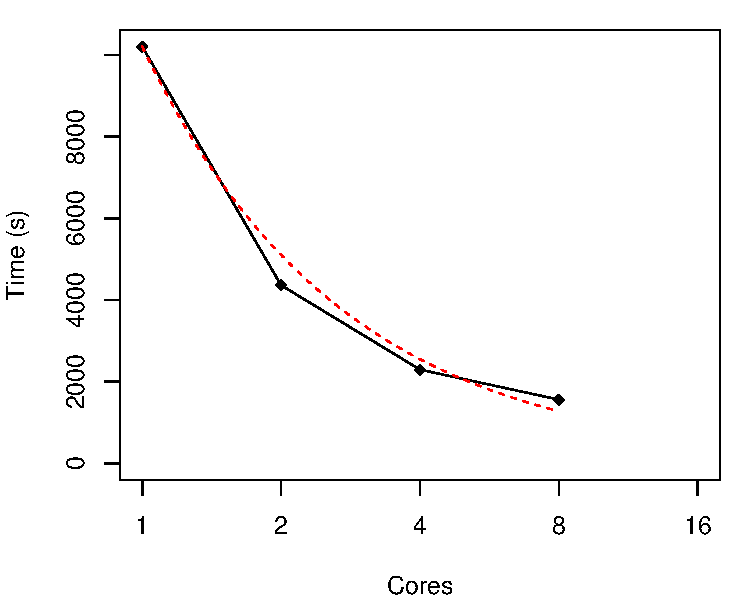
\includegraphics[height=0.8\textheight]{lotkav-iterations-shared-time.pdf}\end{center}
\end{frame}

\begin{frame}{Závěr}
	\begin{itemize}
		\item volně dostupný na internetu (+dokumentace)\\\mbox{\url{https://github.com/sybila/parasim/wiki}}
		\item open-source (GNU GPL)
		\item navazující diplomové práce
			(distribuovaný výpočet, logika s~větší vyjadřovací silou)
	\end{itemize}
\end{frame}

\frame[plain]{}

\begin{frame}{Heuristika}
	\begin{center}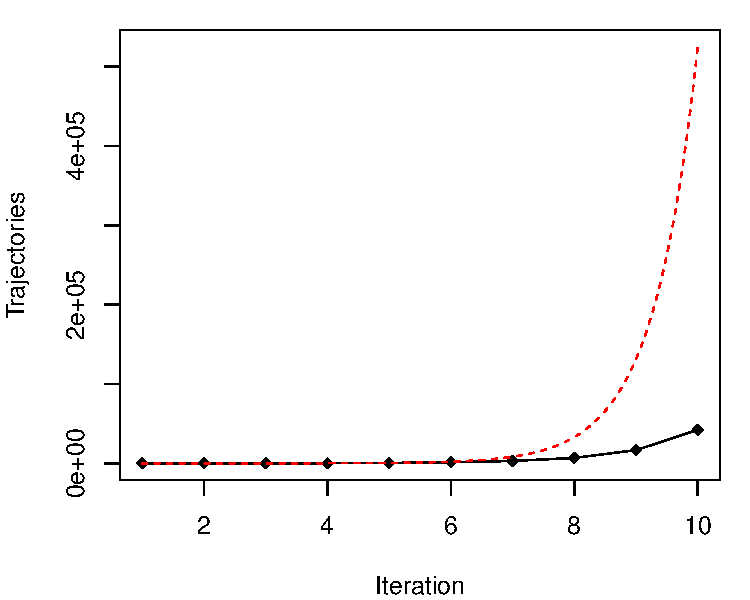
\includegraphics[height=0.9\textheight]{lotkav-iterations-shared-iterations-primary-summary.pdf}\end{center}
\end{frame}

\end{document}
